\subsection*{Tecnologías utilizadas}
	\hfill\break
	\justifying
	El presente documento funciona como reporte de la tarea número 2 asignada en el curso de RFVC.
	
	\hfill\break
	\justifying
	Retomando la infraestructura creada para los objetivos de la primer práctica, se desarrollan los nuevos requisitos del programa añadiendo funcionalidad al programa básico de tratamiento de imágenes.
	
	\hfill\break
	\justifying 
	Se recuerda del primer programa codificado su desarrollo en los lenguajes: Python y QML. Python fue utilizado eclusivamente para los procesos de tratamiento de imágenes, ya sea desarrollando métodos propios o explotando las herramientas disponibles en la biblioteca especializada \textbf{OpenCV}. Así también este lenguaje sirve para la coordinación entre los procesos lógicos y los eventos de la interfaz visual.
	
	\hfill\break
	\justifying
	QML por su parte, como lenguaje de diseño de aplicaciones enfocado en la interfaz de usuario y con un paradigma declarativo, se integra en el \textit{framework} \textbf{PySide6} con soporte para la compatilidad con Python, y que su principal responsabilidad es la de manejar eventos de usuario, actualizaciones de interfaz y demás situaciones relacionadas con la GUI. Utilizando lo que se denomina \textit{Slots}, se logra la ejecución de procesos en el \textit{backend}, y este comunicando a su vez sus resultados con \textit{Signals} hacia la GUI.
	
	\hfill\break
	\justifying
	Del proyecto previo se destacan las funcionalidades disponibles(todas manejables desde un componente en la GUI) que permiten la integración de los nuevos requisitos de esta segunda entrega:
	\begin{itemize}
		\item Apertura imágenes en la GUI para su manejo
		\item Visualizado de los datos de la imagen(Nombre, tamaño en px, formato)
		\item Elección de los colores del pixel en la imagen
		\item Conversión a escala de grises de una imagen
		\item Binarización de la imagén con un umbral especificado
		\item Contabilización de objetos
		\item Recuperado del histograma de la imagen
	\end{itemize}
	
	\subsubsection*{Requisitos para ejecución}
		\begin{itemize}
			\item Python version 3.9.7
			\item Biblioteca \textbf{Numpy}
			\item Biblioteca \textbf{Matplotlib}
			\item Biblioteca \textbf{OpenCV}(4.5.5)
			\item Biblioteca \textbf{PySide6} para la GUI
		\end{itemize}
	
		Una vez instaladas las bibliotecas, dentro de la carpeta de código se puede ejecutar el comando en una terminal:
		
		\begin{verbatim}
 $ python3 main.py
		\end{verbatim}

\subsection*{Objetivo de la práctica}
	\hfill\break
	\justifying
	Implementar funciones básicas del tratamiento de imágenes pertenecientes a etapas de Preprocesamiento y Segmentación, según el paradigma de Gonzalez y Woods.
	
	\hfill\break
	\justifying
	No obligatorio pero si práctico en función de la infraestructura que provee la práctica previa, se integran las nuevas funcionalidades en el programa con interfaz gráfica, facilitando en buena medida su comprensión y uso.
	
	\hfill\break
	\justifying
	Guiándose por los requisitos planteados para esta práctica, se añaden procesos de 6 tareas principalmente, siendo descrito su comportamiento y la solución alcanzada al exponerse a fondo cada una de ellas en su sección particular en páginas siguientes.
	
\subsection*{Interfaz gráfica}
	\hfill\break
	\justifying
	Sin cambios en paleta de colores o estilo de la interfaz, se implementan nuevas secciones colapsables dividiendo las diferentes tareas y sus funciones que se ponen a disposición del usuario.
	\begin{figure}[htbp]
		\centering
		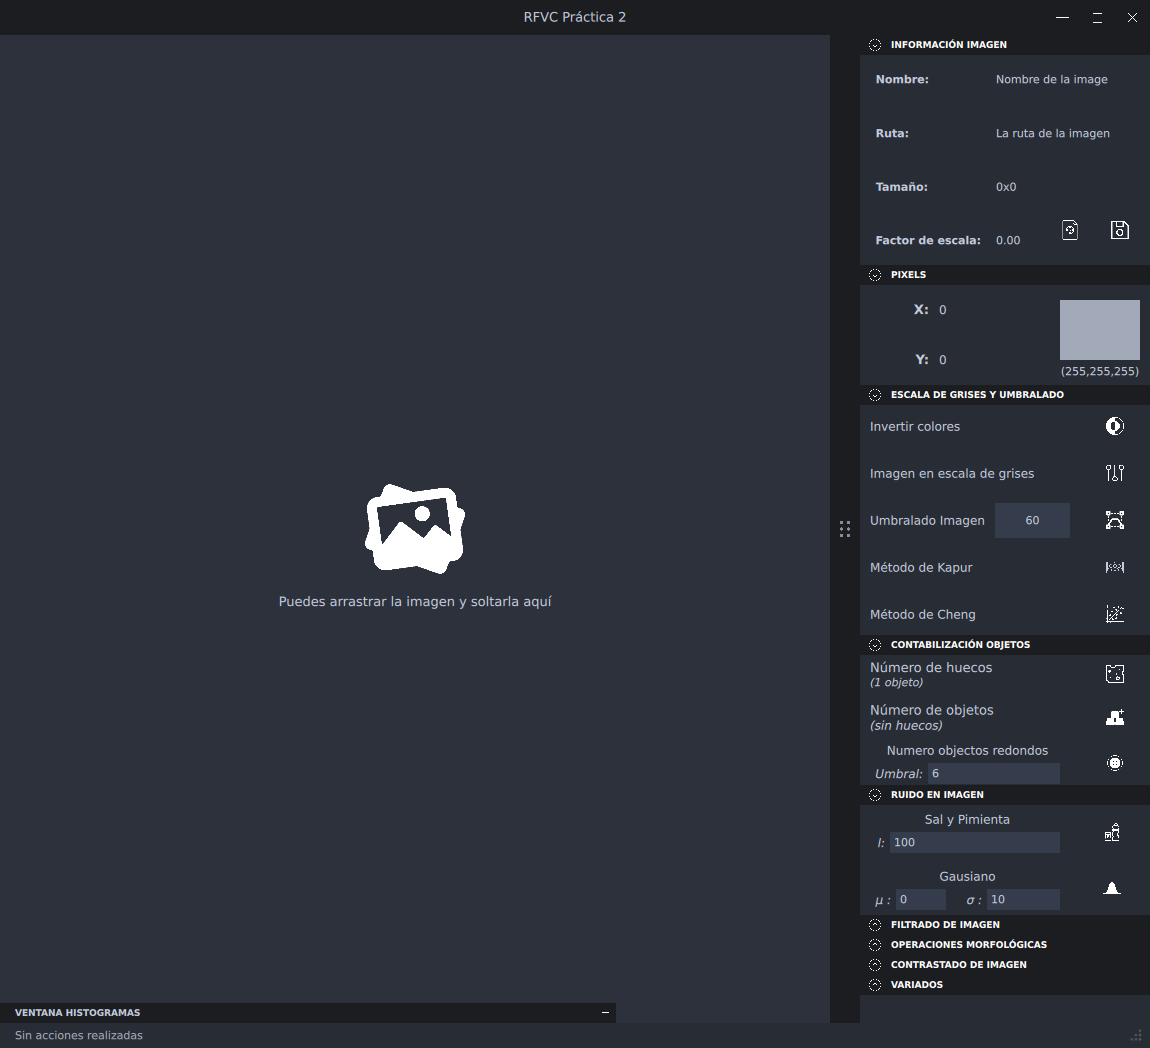
\includegraphics[width=18cm]{Imagenes/GUI.png}
		\caption{Ventana gráfica de la GUI al ejecutarse el programa.}
	\end{figure}
	